\documentclass[aps,prb,10pt,twocolumn,superscriptaddress]{revtex4-2}

\usepackage{tikz,pgf}
\usepackage{amsfonts}
\usepackage{amsmath}
\usepackage{amssymb}
\usepackage{amsthm}
\usepackage{bm}
\usepackage{mathtools}
\usepackage{braket}
\usepackage[right]{lineno}
\usepackage{algorithmicx,algpseudocode}
\usepackage[linesnumbered,ruled,vlined]{algorithm2e}
\usepackage{listings}
\usepackage{subcaption}
\usepackage{caption}
\usepackage{enumitem}
\usepackage{bbm}
\usepackage{graphicx}
\usepackage{array}
\usepackage{booktabs}
\usepackage{float}
\usepackage{hyperref}
\usepackage{xcolor}
\usepackage{todonotes}

\hypersetup{
    colorlinks=true,
    linkcolor=blue,
    citecolor=blue,
    urlcolor=blue
}

\newtheorem{theorem}{Theorem}
\newtheorem{corollary}[theorem]{Corollary}
\newtheorem{remark}[theorem]{Remark}

\newcommand{\placeholderfigure}[2]{%
\begin{figure}[t]
    \centering
    \fbox{\rule{0pt}{2.25in}\rule{0.92\linewidth}{0pt}}
    \caption{#2}
    \label{#1}
\end{figure}
}

\begin{document}

\title{Hybrid Krotov gradient descent Optimization for Quantum Machine Learning}


\author{Maximilian Fröhlich}
\affiliation{Weierstrass Institute for Applied Analysis and Stochastics, Berlin, Germany}
\email{froehlich@wias-berlin.de}
\author{Martin Eigel}
\affiliation{Weierstrass Institute for Applied Analysis and Stochastics, Berlin, Germany}
\author{Michael Hintermüller}
\affiliation{Weierstrass Institute for Applied Analysis and Stochastics, Berlin, Germany}

\date{\today}





\begin{abstract}
We introduce and study a Krotov-inspired discrete adjoint optimization scheme for quantum machine learning and focus on a hybrid online-to-batch schedule. The method transfers the forward/costate/local-update logic of continuous-time optimal control to parameterized quantum circuits by replacing time locality with gate-index locality. For a broad class of fixed-generator variational gates and terminal-state losses, we show that the batch Krotov direction coincides with the exact gradient of the empirical loss. Under standard smoothness assumptions, this yields monotonic descent and convergence of the batch method, and convergence of the tail of the hybrid method after a finite switch to the batch phase. Empirically, we separate two questions. First, on a four-qubit two-moons benchmark, the hybrid schedule explains \emph{why} the method is useful: it combines the fast early progress of online Krotov with the late-stage stability of batch Krotov. Second, on three tuned cross-optimizer benchmarks (HEA on Iris, Simonetti on two-moons, and Chen SUN-VQC on two-moons) we compare hybrid Krotov against Adam, L-BFGS-B, and quantum natural gradient under model-specific hyperparameter sweeps, plus targeted mini-batch-to-full-batch follow-ups for Adam and QNG. The resulting picture is architecture-dependent but consistent: hybrid Krotov is best on the Chen model, statistically tied with the best Adam-family result on Iris, and clearly outperformed by L-BFGS-B on Simonetti; a short hybrid-Adam warmup further improves Simonetti, whereas hybrid QNG brings no advantage. These results position hybrid Krotov as a structured optimizer niche for gate-centric quantum machine learning models rather than as a universal replacement for established first- and second-order methods.
\end{abstract}


\maketitle
\section{Introduction}

Optimization remains one of the main bottlenecks in variational quantum algorithms and quantum machine learning \cite{CerezoEtAl2021VQA,McCleanEtAl2016Theory,MollEtAl2018QST,BiamonteEtAl2017QML,KandalaEtAl2017HEA,McCleanEtAl2018Barren,WangEtAl2021NoiseBP}. In many settings, standard first-order methods provide robust baselines but may converge slowly or require many objective and gradient evaluations, while second-order and quasi-Newton methods can yield strong late-stage refinement but may be more expensive or less naturally aligned with the structure of parameterized quantum circuits. This raises the question whether optimization rules that explicitly exploit circuit propagation structure can offer a useful alternative.

Krotov's method is a classical optimization technique from optimal control \cite{KonnovKrotov1999,WerschnikGross2007,BrifChakrabartiRabitz2010,PalaoKosloff2003,ReichNdongKoch2012,GoerzEtAl2019Krotov}. Its defining ingredients are a forward state trajectory, a backward sensitivity trajectory, and a local update rule derived from the constrained dynamical structure of the problem. In coherent quantum control, these ingredients match the physics especially naturally: the state evolves unitarily, the costate propagates backward through adjoint dynamics, and the update can be written directly in terms of inner products of propagated states and control generators. This motivates the question whether the same logic can be transferred from continuous-time control to gate-structured quantum machine learning models.

In this work we study a discrete, circuit-level adaptation of this idea \cite{SchuldEtAl2019Gradients,BanchiCrooks2021SPSR,WierichsEtAl2022ShiftRules}. The central conceptual move is to replace continuous time by gate index. Forward propagation through the circuit produces a sequence of intermediate states, backward propagation produces a sequence of costates, and local gate-wise update directions are constructed from both. We consider three variants: an online version that updates sample by sample, a batch version that averages sample-wise gate contributions over the dataset, and a hybrid method that uses online updates in an initial phase before switching to batch refinement.

The present paper has two goals. First, it formulates the method in a mathematically clean way and clarifies the extent to which the batch variant can be treated as an exact gradient method. Second, it evaluates whether the hybrid online-to-batch schedule leads to a practically useful optimizer across representative quantum classification benchmarks, including a controlled mechanism study on the original two-moons HEA setting and tuned cross-optimizer comparisons on Iris, Simonetti, and Chen models \cite{SimonettiPerriGervasi2022,SimonettiPerriGervasi2023, ChenEtAl2025SUNVQC}.

The main contributions are as follows.
\begin{itemize}
    \item We formulate a Krotov-inspired discrete adjoint update for parameterized quantum circuits and distinguish carefully between its online, batch, and hybrid variants.
    \item We prove that for fixed-generator variational gates and terminal-state losses, the batch Krotov direction coincides with the exact gradient of the empirical loss.
    \item Under standard smoothness assumptions, we establish monotonic descent and convergence of the batch method, and convergence of the tail of the hybrid method after a finite switch to batch updates.
    \item We clarify the mechanism behind the fast initial loss decrease: the batch Krotov direction is not a hidden alternative descent direction but the exact full-batch gradient, whereas the online phase is a sequential stale-adjoint gate update that performs many local corrections within one epoch. On the original four-qubit two-moons benchmark this yields the clearest mechanistic explanation of the method.
    \item We perform matched hyperparameter sweeps for hybrid Krotov, Adam, L-BFGS-B, and quantum natural gradient on three models, followed by targeted mini-batch-to-full-batch Adam and QNG follow-ups. The tuned comparison shows that the practical value of hybrid Krotov is architecture-dependent: it is best on the Chen model, statistically tied with the best Adam-family result on Iris, and not competitive with L-BFGS-B on Simonetti; the Adam-family follow-up helps only on Simonetti, while hybrid QNG brings no advantage.
\end{itemize}

At the same time, we emphasize from the outset that the present method is not a literal transcription of the classical continuous-time Krotov theorem. The adaptation studied here is best understood as a structured discrete adjoint optimizer for parameterized quantum circuits. The strongest theoretical guarantees in this paper apply to the batch method and to the post-switch phase of the hybrid schedule.

\section{Related Work}

The present work sits at the intersection of quantum optimal control and variational quantum circuit optimization. Its conceptual motivation comes from Krotov-type methods, where a forward state, a backward costate, and a local structure-aware update are coupled through the underlying dynamics. In variational quantum algorithms, by contrast, optimization is usually framed in terms of generic first-order or quasi-Newton updates applied to a black-box objective over circuit parameters. Our contribution is to expose an intermediate viewpoint: the circuit is still discrete and parameterized, but the optimizer can exploit gate-local propagation structure rather than treating the loss as an opaque scalar function.

This structural viewpoint is only meaningful if it is compared against strong modern baselines. We therefore benchmark against Adam, L-BFGS-B, and quantum natural gradient (QNG) \cite{StokesEtAl2020QNG}. Adam serves as the standard adaptive first-order baseline, L-BFGS-B represents quasi-Newton refinement, and QNG adds a geometry-aware natural-gradient baseline. Including all three is important for interpretation: if hybrid Krotov only beat a weak first-order baseline, its scientific value would be limited. The tuned comparisons below instead identify more precisely where the method helps and where it does not.

\section{From continuous-time Krotov to gate-local QML updates}

\subsection{Continuous-time Krotov in optimal control}

Krotov's method originates in constrained optimal control. In the standard setting, a state variable \(\psi(t)\) evolves under a control \(\epsilon(t)\), and one seeks to minimize a cost functional of the form
\begin{equation}
J[\psi,\epsilon]
=
\Phi(\psi(T))
+
\int_0^T g_a(\epsilon(t),t)\,dt
+
\int_0^T g_b(\psi(t),t)\,dt.
\label{eq:generic_cost}
\end{equation}
In coherent quantum dynamics, \(\psi(t)\) often satisfies
\begin{equation}
i \frac{d}{dt}\psi(t)=H(\epsilon(t),t)\psi(t),
\label{eq:schrodinger}
\end{equation}
with prescribed initial condition \(\psi(0)=\psi_0\). Krotov's method constructs a new control \(\epsilon^{(i+1)}(t)\) from a current iterate \(\epsilon^{(i)}(t)\) by combining a forward propagation of the state, a backward propagation of a costate \(\chi(t)\), and a local update rule. A typical schematic form is
\begin{equation}
\epsilon^{(i+1)}(t)
=
\epsilon^{(i)}(t)
+
\frac{S(t)}{\lambda_a}
\operatorname{Im}
\left\langle
\chi^{(i)}(t)
\middle|
\frac{\partial H}{\partial \epsilon}
\middle|
\psi^{(i+1)}(t)
\right\rangle,
\label{eq:krotov_update}
\end{equation}
where \(S(t)\) is a shape function and \(\lambda_a\) is a regularization parameter. The defining conceptual feature is that the update respects the dynamical structure of the problem rather than treating the objective as a black-box function of the control \cite{SklarzTannor2002,PalaoKosloff2003,ReichNdongKoch2012,WerschnikGross2007,BrifChakrabartiRabitz2010}.

\subsection{Parameterized quantum models and terminal-state losses}

In the quantum machine learning setting considered here, the trainable model is a parameterized quantum circuit
\begin{equation}
U(\bm{\theta},x)=U_M(\theta_M,x)\cdots U_1(\theta_1,x),
\label{eq:circuit}
\end{equation}
with trainable parameters \(\bm{\theta}=(\theta_1,\dots,\theta_M)\) and input \(x\). Given a fixed initial state \(|\psi_0\rangle\), the final state for sample \(x_n\) is
\begin{equation}
|\psi_{n,M}(\bm{\theta})\rangle
=
U(\bm{\theta},x_n)|\psi_0\rangle.
\label{eq:final_state}
\end{equation}
We consider binary classification with an empirical loss
\begin{equation}
F(\bm{\theta})=\frac{1}{N}\sum_{n=1}^N L_n(\bm{\theta}),
\qquad
L_n(\bm{\theta})=\ell(p_n(\bm{\theta}),y_n),
\label{eq:empirical_loss}
\end{equation}
where \(p_n(\bm{\theta})\) is the model prediction for sample \(n\), \(y_n\in\{0,1\}\), and \(\ell\) is binary cross-entropy \cite{MitaraiEtAl2018QCL,SchuldEtAl2020CircuitCentric,PerezSalinasEtAl2020DataReupload}.

For a simple one-observable readout, we set
\begin{equation}
z_n(\bm{\theta})
=
\langle \psi_{n,M}(\bm{\theta})|O|\psi_{n,M}(\bm{\theta})\rangle,
\qquad
p_n(\bm{\theta})=\frac{z_n(\bm{\theta})+1}{2}.
\label{eq:simple_readout}
\end{equation}
More generally, if the circuit output is passed into a classical affine head,
\begin{align}
&m_{n,j}
=
\langle \psi_{n,M}(\bm{\theta})|O_j|\psi_{n,M}(\bm{\theta})\rangle,\\
&s_n=\bm{w}^{\top}\bm{m}_n+b, \\
&p_n=\sigma(s_n),
\label{eq:hybrid_head}
\end{align}
then the loss derivative propagates through the classical head before defining the terminal costate \cite{SchuldEtAl2019Gradients,BanchiCrooks2021SPSR,WierichsEtAl2022ShiftRules}.

\subsection{Gate-local forward and backward propagation}

The discrete analogue of continuous-time Krotov is obtained by replacing time locality with gate-index locality. For each sample \(n\), define forward states
\begin{equation}
|\psi_{n,0}\rangle=|\psi_0\rangle,
\qquad
|\psi_{n,k}(\bm{\theta})\rangle
=
U_k(\theta_k,x_n)\cdots U_1(\theta_1,x_n)|\psi_0\rangle,
\label{eq:forward_states}
\end{equation}
for \(k=1,\dots,M\).

Assuming the sample loss depends only on the final state, we define the terminal costate \(|\chi_{n,M}(\bm{\theta})\rangle\) by the first-variation identity
\begin{equation}
\delta L_n(\bm{\theta})
=
2\,\mathrm{Re}\,
\langle \chi_{n,M}(\bm{\theta}) \mid \delta \psi_{n,M}(\bm{\theta}) \rangle.
\label{eq:first_variation}
\end{equation}
For the simple readout \eqref{eq:simple_readout}, this yields
\begin{equation}
|\chi_{n,M}(\bm{\theta})\rangle
=
\frac{1}{2}\frac{\partial \ell}{\partial p_n}
\,O\,|\psi_{n,M}(\bm{\theta})\rangle.
\label{eq:terminal_costate_simple}
\end{equation}
For the hybrid head \eqref{eq:hybrid_head}, one obtains
\begin{equation}
|\chi_{n,M}(\bm{\theta})\rangle
=
(p_n-y_n)
\left(\sum_j w_j O_j\right)
|\psi_{n,M}(\bm{\theta})\rangle.
\label{eq:terminal_costate_hybrid}
\end{equation}

Backward-propagated costates are then defined by
\begin{equation}
|\chi_{n,k}^{\mathrm{after}}(\bm{\theta})\rangle
=
U_{k+1}(\theta_{k+1},x_n)^\dagger \cdots U_M(\theta_M,x_n)^\dagger
|\chi_{n,M}(\bm{\theta})\rangle.
\label{eq:backward_costates}
\end{equation}

\subsection{Online, batch, and hybrid Krotov}

Suppose gate \(k\) is parameterized by a scalar \(\theta_k\) and takes the form
\begin{equation}
U_k(\theta_k,x_n)=\exp\!\left(-\frac{i}{2}\alpha_k(\theta_k,x_n)G_k\right),
\label{eq:fixed_generator_gate}
\end{equation}
where \(G_k\) is a fixed Hermitian generator. The corresponding gate-local contribution for sample \(n\) is
\begin{equation}
\Delta_{n,k}(\bm{\theta})
=
\frac{\partial \alpha_k}{\partial \theta_k}(\theta_k,x_n)\,
2\,\mathrm{Re}\!\left\langle
\chi_{n,k}^{\mathrm{after}}(\bm{\theta})
\middle|
\left(-\frac{i}{2}G_k\right)
\middle|
\psi_{n,k}(\bm{\theta})
\right\rangle.
\label{eq:discrete_contribution}
\end{equation}

This can be interpreted as a generalization of the reverse-mode gradient derived in \cite{jones2020efficientcalculationgradientsclassical} and yields the same computational advantage in full quantum state simulation compared to parameter-shift rule .

For fixed \(\bm{\theta}\), the quantity \(\Delta_{n,k}(\bm{\theta})\) is exactly the sample-wise partial derivative \(\partial L_n/\partial \theta_k\). The distinction between the online and batch variants is therefore not the local formula itself, but how this formula is reused during an update sweep.

We consider three algorithmic variants.

\paragraph{Online Krotov.}
For one training sample \((x_n,y_n)\), we compute the forward states and backward costates once at a current parameter vector \(\bm{\theta}^{\mathrm{old}}\), then update parameters gate by gate. If \(|\tilde{\psi}_{n,k-1}\rangle\) denotes the forward state obtained after updating gates \(1,\dots,k-1\) within the same sample, the implemented gate-\(k\) online signal has the mixed stale/fresh form
\begin{equation}
\widehat{\Delta}_{n,k}
=
\frac{\partial \alpha_k}{\partial \theta_k}(\theta_k^{\mathrm{old}},x_n)\,
2\,\mathrm{Re}\!\left\langle
\chi_{n,k}^{\mathrm{after}}(\bm{\theta}^{\mathrm{old}})
\middle|
\left(-\frac{i}{2}G_k\right)
\middle|
U_k(\theta_k^{\mathrm{old}},x_n)\tilde{\psi}_{n,k-1}
\right\rangle,
\label{eq:online_mixed_signal}
\end{equation}
followed by \(\theta_k \leftarrow \theta_k-\eta_{\mathrm{on}}\widehat{\Delta}_{n,k}\). Thus the backward trajectory is fully stale, whereas the forward trajectory is refreshed gate by gate within the sample. This variant is aggressive and often effective in the early training regime, but it may induce substantial late-stage oscillations.

\paragraph{Batch Krotov.}
We average the sample-wise contributions over the dataset,
\begin{equation}
\bar{\Delta}_k(\bm{\theta})
=
\frac{1}{N}\sum_{n=1}^N \Delta_{n,k}(\bm{\theta}),
\label{eq:batch_direction}
\end{equation}
and perform a single parameter update
\begin{equation}
\theta_k^{(m+1)}=\theta_k^{(m)}-\eta\,\bar{\Delta}_k(\bm{\theta}^{(m)}).
\label{eq:batch_update}
\end{equation}
This is more stable than the online rule and aligns directly with the empirical loss.

\paragraph{Hybrid Krotov.}
The hybrid method uses online Krotov for an initial phase \(m<T_{\mathrm{sw}}\) and switches to batch Krotov for \(m\geq T_{\mathrm{sw}}\). The intended effect is to combine rapid basin entry with stable late-stage refinement.

\paragraph{Non-gate parameters.}
For hybrid quantum-classical models, purely classical parameters such as \(\bm{w}\) and \(b\) in \eqref{eq:hybrid_head} are not updated by the gate-local Krotov rule. In the experiments below, such parameters receive their exact loss-gradient update within the same training epoch.

\paragraph{Optional discrete scaling factors.}
The continuous-time update \eqref{eq:krotov_update} contains the multiplicative factor \(S(t)/\lambda_a\). In the discrete implementation this motivates optional per-gate factors \(S_k\) of the form
\begin{equation}
\theta_k^{+}
=
\theta_k-\eta S_k \widehat{\Delta}_{n,k}
\qquad\text{or}\qquad
\theta_k^{+}
=
\theta_k-\eta S_k \bar{\Delta}_k,
\label{eq:discrete_scaling}
\end{equation}
depending on whether the phase is online or batch. We tested both adaptive choices, where \(S_k\) depends on the current update magnitude, and metadata-based choices, where \(S_k\) depends on layer or parameter group. These factors should be interpreted as heuristic preconditioners rather than as part of the exact-gradient theory; the convergence results below apply to the unscaled batch rule.

\section{Theoretical properties}

The main theoretical message of this paper is deliberately modest. We do not claim that the present discrete QML adaptation inherits the full classical continuous-time Krotov theorem. Instead, we prove three precise statements:
\begin{enumerate}
    \item for fixed-generator gates and terminal-state losses, the batch Krotov direction is the exact gradient of the empirical loss;
    \item under standard smoothness assumptions, the batch method is a monotone gradient-descent scheme and converges to stationary points;
    \item the tail of the hybrid method converges after a finite switch to batch Krotov.
\end{enumerate}

\begin{theorem}[Exact gradient representation of the batch Krotov direction]
\label{thm:exact_gradient_krotov_main}
Let \(F(\bm{\theta})\) be defined by \eqref{eq:empirical_loss}, assume that each trainable gate has the fixed-generator form \eqref{eq:fixed_generator_gate}, and assume that each sample loss depends on the circuit only through the final state. Then the batch Krotov direction \(\bar{\Delta}(\bm{\theta})\) defined by \eqref{eq:batch_direction} coincides with the exact gradient of the empirical loss:
\[
\bar{\Delta}(\bm{\theta})=\nabla F(\bm{\theta}).
\]
\end{theorem}

\begin{theorem}[Monotonic descent and convergence of batch Krotov]
\label{thm:batch_krotov_convergence_main}
Assume that the batch Krotov direction equals \(\nabla F\), that \(F\) is bounded below, and that \(F\) is \(L\)-smooth on the relevant sublevel set. Consider the batch iteration
\[
\bm{\theta}^{(m+1)}=\bm{\theta}^{(m)}-\eta \nabla F(\bm{\theta}^{(m)})
\]
with fixed step size \(0<\eta<2/L\). Then \(F(\bm{\theta}^{(m)})\) is monotonically nonincreasing and
\[
F(\bm{\theta}^{(m+1)})
\leq
F(\bm{\theta}^{(m)})
-\eta\left(1-\frac{L\eta}{2}\right)\|\nabla F(\bm{\theta}^{(m)})\|^2.
\]
Moreover,
\[
\sum_{m=0}^{\infty}\|\nabla F(\bm{\theta}^{(m)})\|^2<\infty,
\qquad
\|\nabla F(\bm{\theta}^{(m)})\|\to 0,
\]
and every accumulation point is stationary. If, in addition, the iterates are bounded and \(F\) satisfies the Kurdyka--\L{}ojasiewicz property, then the whole sequence converges to a single stationary point.
\end{theorem}

\begin{corollary}[Convergence of the tail of hybrid Krotov]
\label{cor:hybrid_tail_main}
Assume that the iterates are generated by an arbitrary online Krotov phase for \(m<T_{\mathrm{sw}}\), and by batch Krotov for \(m\geq T_{\mathrm{sw}}\), with a finite switch time \(T_{\mathrm{sw}}<\infty\) and a step size satisfying \(0<\eta<2/L\). Under the assumptions of Theorem~\ref{thm:batch_krotov_convergence_main}, the tail sequence \((\bm{\theta}^{(m)})_{m\geq T_{\mathrm{sw}}}\) converges to a stationary point under the same boundedness and Kurdyka--\L{}ojasiewicz assumptions.
\end{corollary}

The proofs are given in Appendix~A and Appendix~B. The practical interpretation is important. The theoretical guarantees established here apply to the batch method and to the post-switch phase of the hybrid method. They do \emph{not} imply a monotonic-descent theorem for the online stale-adjoint phase, which empirically is precisely the regime where oscillations are observed.

\section{Why the online phase can decrease the loss quickly}

Theorem~\ref{thm:exact_gradient_krotov_main} has an immediate interpretive consequence. For gate-supported parameters, the batch Krotov direction is already the exact gradient of the empirical loss. Hence the fast initial improvement observed for hybrid Krotov cannot be explained by a hidden superior batch descent direction. The mechanism must lie in the online phase and in the way that phase reuses forward and backward information.

Equation~\eqref{eq:online_mixed_signal} shows that the implemented online rule is a mixed stale/fresh update. For the first gate of a given sample, the signal coincides with the exact sample gradient at the current parameter vector. After that first gate update, however, the forward state has already been modified while the backward costates are still those of the old parameters. The online phase is therefore best understood as a sequential Gauss--Seidel-like discrete adjoint sweep rather than as simultaneous gradient descent.

This has a simple but important algorithmic consequence. With \(N\) training samples and \(K\) gate-supported parameters, one online epoch performs \(N\times K\) local parameter modifications, because each sample triggers a full gate sweep. By contrast, the batch rule aggregates all samples before a single outer update. The online phase therefore has much finer within-epoch resolution: corrections made at early gates immediately affect the forward states seen by later gates in the same sample, and the next sample starts from the already-updated parameter vector.

This finer resolution does not require \(N\times K\) fresh adjoint recomputations. For a fixed sample, the online rule forms one forward trajectory and one backward costate trajectory and then reuses them across the whole gate sweep, so the additional gate-local corrections are mostly cheap local linear-algebra operations rather than new propagation passes. In the cost accounting used in this paper, online Krotov therefore spends roughly one sample forward pass plus one sample backward pass per training sample and amortizes that information over many sequential local updates. Adam and full-batch Krotov, by contrast, spend a full-batch forward/backward evaluation to construct one averaged update direction at the current parameter vector, while L-BFGS-B may require several such full-batch evaluations because of its line-search and quasi-Newton bookkeeping.

The price of this granularity is that the online signal is no longer the exact coordinate gradient of the current partially updated parameter vector. Under local smoothness, the mismatch between \(\widehat{\Delta}_{n,k}\) and the exact coordinate gradient after the previous intra-sample updates is controlled by the accumulated earlier gate changes, so the discrepancy is largest when the online updates are large and shrinks as the trajectory settles. We interpret this as an implicit gradient perturbation of the sequential rule, not as a proved monotonicity mechanism. In particular, the classical continuous-time Krotov theorem does not transfer to this stale-adjoint online phase.

At the sample level, the method also behaves like a structured stochastic optimizer: training samples are processed in random order, and each sample sees parameters left behind by the previous one. The online phase thus combines sample-wise stochasticity with gate-wise sequentiality. This is exactly the behavior that the switch and hyperparameter sweeps below probe. Our expectation, confirmed empirically, is that the decisive knobs are the duration of the online phase and the relative scales of the online and batch step sizes, whereas additional discrete scaling factors \(S_k\) can only provide secondary refinements.

\section{Numerical experiments}

\subsection{Experimental design}

We report three complementary empirical protocols.
First, we revisit the original four-qubit hardware-efficient two-moons benchmark and use it as a \emph{mechanism study}: here the main question is why the hybrid schedule helps relative to pure online and pure batch Krotov.
Second, we add a binary Iris benchmark using the same four-qubit HEA to test whether the optimizer behavior generalizes beyond the two-moons geometry.
Third, we perform matched hyperparameter sweeps for all four optimizers on three models: HEA on Iris, the full Simonetti--Perri--Gervasi hybrid classifier on two-moons, and the improved Chen SUN-VQC on two-moons.

The fixed-setting benchmark figures and the tuned summary tables serve different purposes and should be read accordingly.
The fixed-setting figures show the characteristic optimization dynamics of the method.
The tuned tables answer the fairer question of which optimizer performs best once each method is allowed to use sensible model-specific hyperparameters.

Throughout, we report not only iteration count and wall-clock time, but also a fair propagation-cost axis defined by
\[
\text{cost units}
=
\text{sample forward passes}
+
\text{sample backward passes}.
\]

\subsection{Main two-moons benchmark: why the hybrid schedule helps}

We first consider the original four-qubit HEA two-moons benchmark.
The setup uses four qubits, three trainable layers, five random seeds, and one hundred outer iterations on a fixed train/test split.
The comparison includes online Krotov, batch Krotov, hybrid Krotov, Adam, and L-BFGS-B.
This subsection is intentionally not the final word on overall optimizer ranking; it is the cleanest benchmark for isolating the schedule effect itself.

Table~\ref{tab:main_benchmark} already shows the central mechanism.
Pure online Krotov reaches the loss threshold \(0.40\) almost immediately but exhibits substantial late-stage oscillations.
Pure batch Krotov is far more stable but loses the early-time advantage.
The hybrid schedule combines both features: it preserves the fast threshold crossing of online Krotov while substantially reducing the late-stage oscillation and improving final training loss.

\begin{table}[H]
\centering
\resizebox{\linewidth}{!}{%
\begin{tabular}{lcccccc}
\toprule
Optimizer & Final loss & Final test acc. & Wall time (s) & Time to \(\leq 0.40\) (s) & Success @ 0.40 & Tail std. \\
\midrule
Krotov online & \(0.354 \pm 0.011\) & \(0.839 \pm 0.012\) & \(22.8 \pm 2.9\) & 1.2 & 1.00 & 0.0341 \\
Krotov batch & \(0.365 \pm 0.036\) & \(0.852 \pm 0.015\) & \(65.0 \pm 0.9\) & 26.8 & 0.80 & 0.0024 \\
Hybrid sw\(=10\) & \(0.329 \pm 0.012\) & \(0.841 \pm 0.023\) & \(58.2 \pm 11.1\) & 1.1 & 1.00 & 0.0001 \\
Adam & \(0.355 \pm 0.041\) & \(0.868 \pm 0.025\) & \(67.4 \pm 3.8\) & 26.6 & 0.80 & 0.0009 \\
L-BFGS-B & \(0.321 \pm 0.012\) & \(0.848 \pm 0.021\) & \(47.8 \pm 8.8\) & 9.7 & 1.00 & 0.0001 \\
\bottomrule
\end{tabular}
}
\caption{Main comparison on the aligned five-seed four-qubit two-moons benchmark.}
\label{tab:main_benchmark}
\end{table}

The fairest interpretation of this table is not that hybrid Krotov dominates every baseline on every metric.
L-BFGS-B still yields the best final loss, and Adam attains the highest mean final test accuracy.
The strongest statement supported by the data is narrower and more interesting: hybrid Krotov gives the best combination of rapid early progress and stable late-stage training among the Krotov-family methods, clearly improves over Adam in time-to-threshold and final training loss in this protocol, and remains competitive with L-BFGS-B while using a structured gate-local update.

\begin{figure}[H]
\centering

\includegraphics[width=0.8\linewidth]{figures/comparison_loss_vs_iteration.pdf}
\caption{Training loss versus iteration for the main comparison, with the best hybrid variant substituted for the generic hybrid family.}
\label{fig:main_loss_iteration}
\end{figure}

\begin{figure}[H]
\centering

\includegraphics[width=0.8\linewidth]{figures/comparison_loss_vs_time.pdf}
\caption{Training loss versus wall-clock time. The hybrid closes the final-loss gap without sacrificing the practical runtime advantage.}
\label{fig:main_loss_time}
\end{figure}

\begin{figure}[H]
\centering

\includegraphics[width=0.8\linewidth]{figures/comparison_loss_vs_cost.pdf}
\caption{Training loss versus fair propagation cost. The hybrid inherits the rapid early threshold crossing of the online rule while remaining as propagation-efficient as the other Krotov-family methods.}
\label{fig:main_loss_cost}
\end{figure}

\begin{figure}[H]
\centering

\includegraphics[width=0.8\linewidth]{figures/time_to_threshold_boxplot.pdf}
\caption{Wall-clock time to reach the benchmark threshold loss \(\leq 0.40\).}
\label{fig:main_threshold}
\end{figure}

\subsection{From switch sweep to full hybrid tuning}

To study the role of the hybrid schedule itself, we vary the switching iteration over
\[
T_{\mathrm{sw}}\in \{5,10,20,30,50\}.
\]
The results are summarized in Table~\ref{tab:switch_sweep}. The outcome is unusually clean. Very late switches revert toward the noisy online behavior, while earlier switches perform best. In the present benchmark, switching at \(10\) gives the strongest final loss, while switching at \(5\) gives the best overall wall-clock runtime among the tested hybrid settings.

\begin{table}[H]
\centering
\begin{tabular}{lcccc}
\toprule
Hybrid setting & Final loss & Wall time (s) & Time to \(\leq 0.40\) (s) & Tail std. \\
\midrule
Hybrid sw\(=5\) & \(0.332 \pm 0.013\) & 48.1 & 1.1 & 0.0025 \\
Hybrid sw\(=10\) & \(0.329 \pm 0.012\) & 58.2 & 1.1 & 0.0001 \\
Hybrid sw\(=20\) & \(0.346 \pm 0.014\) & 27.2 & 1.1 & 0.0183 \\
Hybrid sw\(=30\) & \(0.354 \pm 0.011\) & 21.3 & 1.1 & 0.0341 \\
Hybrid sw\(=50\) & \(0.354 \pm 0.011\) & 21.5 & 1.1 & 0.0341 \\
\bottomrule
\end{tabular}
\caption{Switch sweep for hybrid Krotov on the main benchmark.}
\label{tab:switch_sweep}
\end{table}

These results support a specific mechanistic interpretation. Online Krotov appears to act as a short, high-gain transient that moves parameters quickly into a good basin. If left active for too long, it induces unnecessary late-stage movement. Batch Krotov, by contrast, is well suited to stable refinement once the trajectory is already close to a good classifier. The hybrid method works because it assigns each update regime to the stage of training where it is strongest.

The later sweep study shows, however, that the switch alone is not the whole story.
Across models, the best hybrid performance depends jointly on the switching time and the online and batch step sizes.
The simple switch sweep is therefore best understood as a first mechanism study, not as a complete tuning analysis.

\begin{figure}[H]
\centering
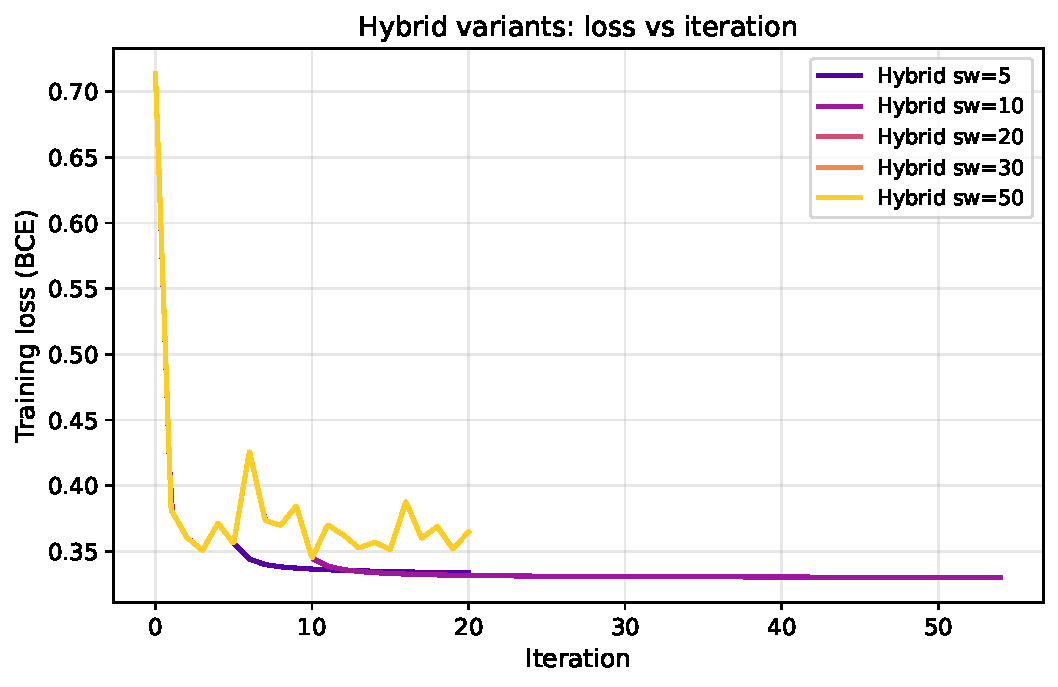
\includegraphics[width=0.82\linewidth]{figures/hybrid_switch_loss_vs_iteration.pdf}
\caption{Loss versus iteration for the hybrid switch sweep. Very late switches drift back toward the noisier online behavior.}
\label{fig:switch_loss_iteration}
\end{figure}

\begin{figure}[H]
\centering
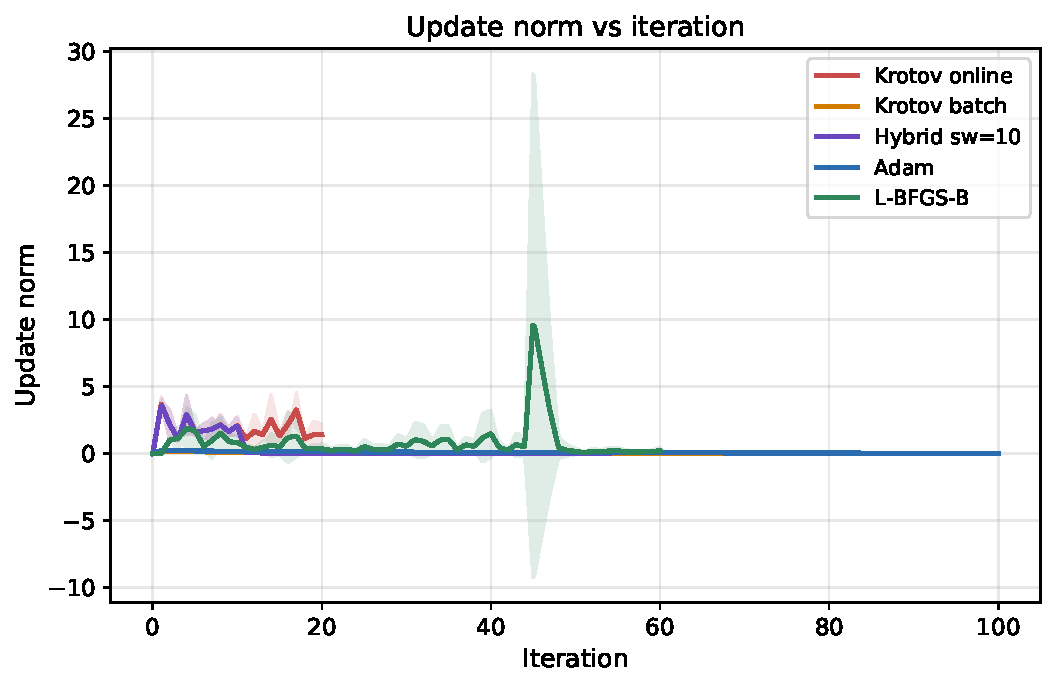
\includegraphics[width=0.8\linewidth]{figures/comparison_update_norm_vs_iteration.pdf}
\caption{Update norms for the main comparison. The hybrid retains a strong early move and then settles into a batch-like refinement regime.}
\label{fig:update_norms}
\end{figure}

\begin{figure}[H]
\centering
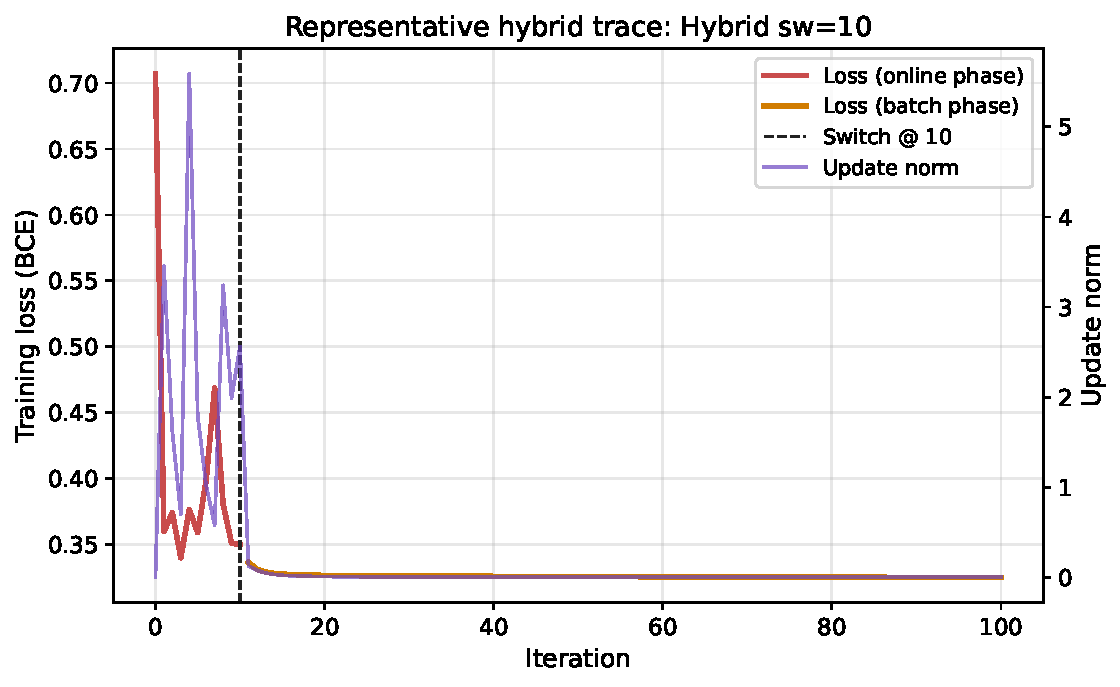
\includegraphics[width=0.8\linewidth]{figures/hybrid_phase_transition_trace.pdf}
\caption{Representative hybrid trace with the phase transition marked explicitly. The loss flattens rapidly after the switch while update norms collapse.}
\label{fig:phase_transition}
\end{figure}

\begin{figure}[H]
\centering

\includegraphics[width=\linewidth]{figures/comparison_decision_boundaries.pdf}
\caption{Representative decision boundaries for the main comparison.}
\label{fig:decision_boundaries_main}
\end{figure}

\subsection{Iris HEA benchmark}

To test whether the optimizer behavior generalizes beyond the two-moons geometry, we add a binary Iris benchmark using the same four-qubit, three-layer HEA architecture.
The dataset is restricted to setosa versus versicolor, uses the first two features, and is scaled to \([0,\pi]\) for angle encoding.
The protocol uses five random seeds and one hundred outer iterations.

\begin{table}[H]
\centering
\resizebox{\linewidth}{!}{%
\begin{tabular}{lcccccc}
\toprule
Optimizer & Final loss & Final test acc. & Wall time (s) & Time to \(\leq 0.40\) (s) & Success @ 0.40 & Tail std. \\
\midrule
Hybrid Krotov & \(0.255 \pm 0.025\) & \(0.980 \pm 0.024\) & \(18.6 \pm 1.1\) & 0.3 & 1.00 & 0.0000 \\
Adam & \(0.273 \pm 0.023\) & \(0.970 \pm 0.024\) & \(17.0 \pm 0.7\) & 3.4 & 1.00 & 0.0017 \\
L-BFGS-B & \(0.263 \pm 0.018\) & \(0.980 \pm 0.024\) & \(7.4 \pm 1.2\) & 0.9 & 1.00 & 0.0000 \\
QNG & \(0.267 \pm 0.022\) & \(0.970 \pm 0.024\) & \(39.7 \pm 0.3\) & 2.4 & 1.00 & 0.0001 \\
\bottomrule
\end{tabular}}
\caption{Binary Iris HEA benchmark under a fixed-setting protocol (5 seeds, 100 iterations). QNG uses learning rate 0.5 and metric regularization \(\lambda=0.01\).}
\label{tab:iris_benchmark}
\end{table}

Under this fixed-setting protocol, all four optimizers converge to strong classifiers.
Hybrid Krotov attains the lowest mean final loss and the fastest threshold crossing, while L-BFGS-B is by far the fastest in wall-clock time overall.
QNG reaches a comparable final loss but at a noticeably higher runtime because of the metric-tensor overhead.
This Iris result is important for the paper narrative because it shows that the method is not tied to one synthetic two-moons setup.

\begin{figure}[H]
\centering
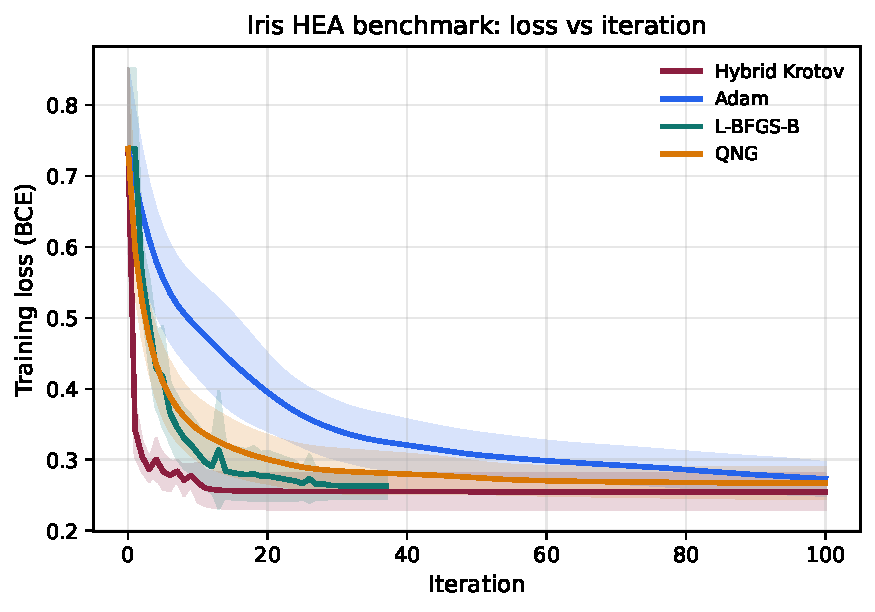
\includegraphics[width=0.8\linewidth]{figures/loss_vs_iteration.pdf}
\caption{Iris HEA benchmark: mean training loss versus iteration for Hybrid Krotov, Adam, L-BFGS-B, and QNG.}
\label{fig:iris_loss_iteration}
\end{figure}

\begin{figure}[H]
\centering

\includegraphics[width=\linewidth]{figures/decision_boundaries.pdf}
\caption{Iris HEA benchmark: representative decision boundaries. All optimizers learn a clean separator; the differences are mainly in convergence speed and final calibration.}
\label{fig:iris_boundaries}
\end{figure}

\subsection{Cross-optimizer comparison after hyperparameter tuning}

The strongest empirical question is not which optimizer wins under one hand-chosen setting, but which wins after each method is given a reasonable tuning budget.
We therefore swept the relevant hyperparameters of all four optimizers on three models:
\begin{itemize}
    \item Hybrid Krotov: switch iteration, online step size, batch step size;
    \item Adam: learning rate;
    \item L-BFGS-B: history size \texttt{maxcor} and gradient tolerance \texttt{gtol};
    \item QNG: learning rate and Tikhonov regularization parameter \(\lambda\).
\end{itemize}
Each configuration was evaluated with three random seeds.
For hybrid Krotov and Adam, an additional extended grid was run whenever the default sweep suggested a promising boundary region.
After these matched sweeps, we ran a targeted follow-up motivated by the hybrid-Krotov mechanism: Adam and QNG were allowed to use a short mini-batch phase before reverting to their standard full-batch updates.
Only one case improved on the best previously tested baseline, namely Simonetti with hybrid Adam at learning rate \(0.3\), batch size \(32\), and switch \(T_{\mathrm{sw}}=5\), which reduced the mean final loss to \(0.0126 \pm 0.0004\) over two follow-up seeds.
The corresponding hybrid-QNG trials brought no advantage on any tested model, and we did not pursue an analogous hybrid L-BFGS-B variant because stochastic gradients are a poor match to quasi-Newton curvature memory; such a procedure would be better interpreted as a separate warm-start protocol rather than as a direct optimizer variant.

\begin{table*}[t]
\centering
\small
\begin{tabular}{>{\raggedright\arraybackslash}p{2.6cm}
                >{\centering\arraybackslash}p{2.7cm}
                >{\centering\arraybackslash}p{2.7cm}
                >{\centering\arraybackslash}p{2.7cm}
                >{\centering\arraybackslash}p{2.7cm}}
\toprule
Model & Hybrid Krotov & Adam & L-BFGS-B & QNG \\
\midrule
HEA (Iris)
  & \shortstack{\(0.2424 \pm 0.015\)\\test acc.\ 0.983}
  & \shortstack{\(\mathbf{0.2397 \pm 0.011}\)\\test acc.\ 1.000}
  & \shortstack{\(0.2655 \pm 0.008\)\\test acc.\ 0.983}
  & \shortstack{\(0.2802 \pm 0.013\)\\test acc.\ 1.000} \\
Simonetti
  & \shortstack{\(0.0358 \pm 0.001\)\\test acc.\ 1.000}
  & \shortstack{\(0.0126 \pm 0.0004\)\\test acc.\ 1.000}
  & \shortstack{\(\mathbf{0.0007 \pm 0.001}\)\\test acc.\ 1.000}
  & \shortstack{\(0.0501 \pm 0.004\)\\test acc.\ 1.000} \\
Chen SUN-VQC
  & \shortstack{\(\mathbf{0.3828 \pm 0.010}\)\\test acc.\ 0.989}
  & \shortstack{\(0.4138 \pm 0.014\)\\test acc.\ 0.956}
  & \shortstack{\(0.3933 \pm 0.011\)\\test acc.\ 0.983}
  & \shortstack{\(0.3991 \pm 0.004\)\\test acc.\ 0.989} \\
\bottomrule
\end{tabular}
\caption{Best result for each optimizer family on each model. The Simonetti Adam entry comes from a targeted two-seed hybrid-Adam follow-up (\(B=32\), \(T_{\mathrm{sw}}=5\)) because it improved over the best pure-Adam sweep; the hybrid-QNG follow-ups did not improve any table entry. On HEA (Iris), Adam and Hybrid Krotov are within one standard deviation and should be treated as statistically tied on final loss.}
\label{tab:tuned_cross_model}
\end{table*}

\begin{table*}[t]
\centering
\small
\begin{tabular}{>{\raggedright\arraybackslash}p{2.7cm}
                >{\raggedright\arraybackslash}p{2.9cm}
                >{\raggedright\arraybackslash}p{2.2cm}
                >{\raggedright\arraybackslash}p{2.4cm}
                >{\raggedright\arraybackslash}p{2.4cm}}
\toprule
Model & Hybrid Krotov & Adam & L-BFGS-B & QNG \\
\midrule
HEA (Iris)
  & sw\(=20\), online\(=1.0\), batch\(=3.0\)
  & lr\(=1.0\)
  & maxcor\(=20\), gtol\(=10^{-8}\)
  & lr\(=1.0\), \(\lambda=0.1\) \\
Simonetti
  & sw\(=5\), online\(=0.2\), batch\(=1.0\)
  & lr\(=0.3\), batch\(=32\), sw\(=5\)
  & maxcor\(=10\), gtol\(=10^{-5}\)
  & lr\(=1.0\), \(\lambda=0.001\) \\
Chen SUN-VQC
  & sw\(=15\), online\(=0.1\), batch\(=0.3\)
  & lr\(=0.2\)
  & maxcor\(=10\), gtol\(=10^{-5}\)
  & lr\(=0.5\), \(\lambda=0.01\) \\
\bottomrule
\end{tabular}
\caption{Best hyperparameters identified by the sweeps, augmented by the targeted Simonetti hybrid-Adam follow-up. Only the Simonetti Adam-family entry uses a mini-batch warmup; the hybrid-QNG follow-ups did not improve over the full-batch sweep settings.}
\label{tab:best_hparams}
\end{table*}

The tuned comparison changes the empirical story in three important ways.
First, it removes the ambiguity between optimizer quality and poor hyperparameter choice.
Second, it reveals strong model dependence.
Third, it shows that the original mechanistic story about the hybrid schedule remains useful, but only as part of a larger optimizer picture.

For HEA on Iris, the fixed-setting benchmark in Table~\ref{tab:iris_benchmark} shows Hybrid Krotov as the fastest threshold-crosser and the best mean final-loss method.
After tuning, however, Adam at learning rate \(1.0\) and Hybrid Krotov at \((T_{\mathrm{sw}},\eta_{\mathrm{on}},\eta_{\mathrm{bat}})=(20,1.0,3.0)\) are within one standard deviation of each other.
This is exactly the kind of correction that strengthens the paper: the method still looks strong, but the claim becomes more precise and more defensible.

For the full Simonetti hybrid classifier, tuning changes the interpretation of Hybrid Krotov substantially.
Under untuned or lightly tuned settings, Hybrid Krotov looked clearly weaker than the best baselines.
After tuning, its final loss improves dramatically to \(0.0358 \pm 0.001\), which is a large absolute gain over the earlier fixed-setting value \(0.448 \pm 0.055\).
A targeted hybrid-Adam follow-up then improves the Adam-family result further to \(0.0126 \pm 0.0004\) at \((\eta,B,T_{\mathrm{sw}})=(0.3,32,5)\), compared with \(0.0211 \pm 0.006\) for the best pure-Adam sweep.
Even so, L-BFGS-B remains decisively best at \(0.0007 \pm 0.001\).
The correct conclusion is therefore not that Hybrid Krotov fails on Simonetti, but that Simonetti strongly favors quasi-Newton refinement and also benefits from a short Adam-family warm-start schedule once the hybrid classical head is restored.

For the Chen SUN-VQC, the tuned comparison is the strongest evidence for the project hypothesis.
Here Hybrid Krotov becomes the best optimizer overall, reaching \(0.3828 \pm 0.010\), ahead of L-BFGS-B at \(0.3933 \pm 0.011\), QNG at \(0.3991 \pm 0.004\), and Adam at \(0.4138 \pm 0.014\).
By contrast with Simonetti, the hybrid-Adam follow-up does not change the Chen ranking: the best tested short-warmup Adam variant reaches \(0.4315 \pm 0.027\) over two seeds, essentially matching but not improving the best pure-Adam sweep and remaining clearly behind Hybrid Krotov.
The hybrid-QNG follow-ups are also worse than the best full-batch QNG settings on all tested models.
This is precisely the kind of genuinely gate-centric regime in which a structured circuit-aware update can plausibly pay off.

\begin{figure}[t]
\centering
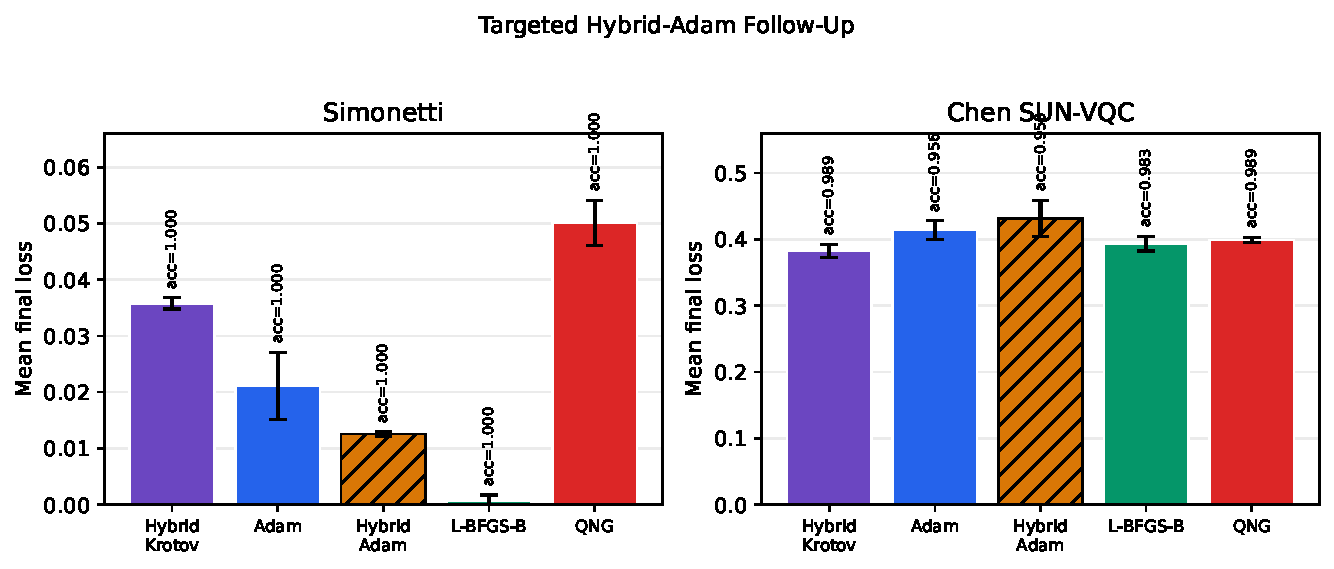
\includegraphics[width=0.95\linewidth]{figures/adam_hybrid_followup.pdf}
\caption{Targeted hybrid-Adam follow-up on Simonetti and Chen. A short mini-batch-to-full-batch warmup improves the Simonetti Adam-family result substantially, but does not improve Chen. Hybrid-Adam bars summarize the two-seed follow-up runs; the other bars reproduce the best tuned results from Table~\ref{tab:tuned_cross_model}. Hybrid-QNG follow-ups are omitted because they brought no advantage on any tested model.}
\label{fig:hybrid_adam_followup}
\end{figure}

\begin{figure*}[t]
\centering
\begin{subfigure}{0.32\textwidth}
\centering
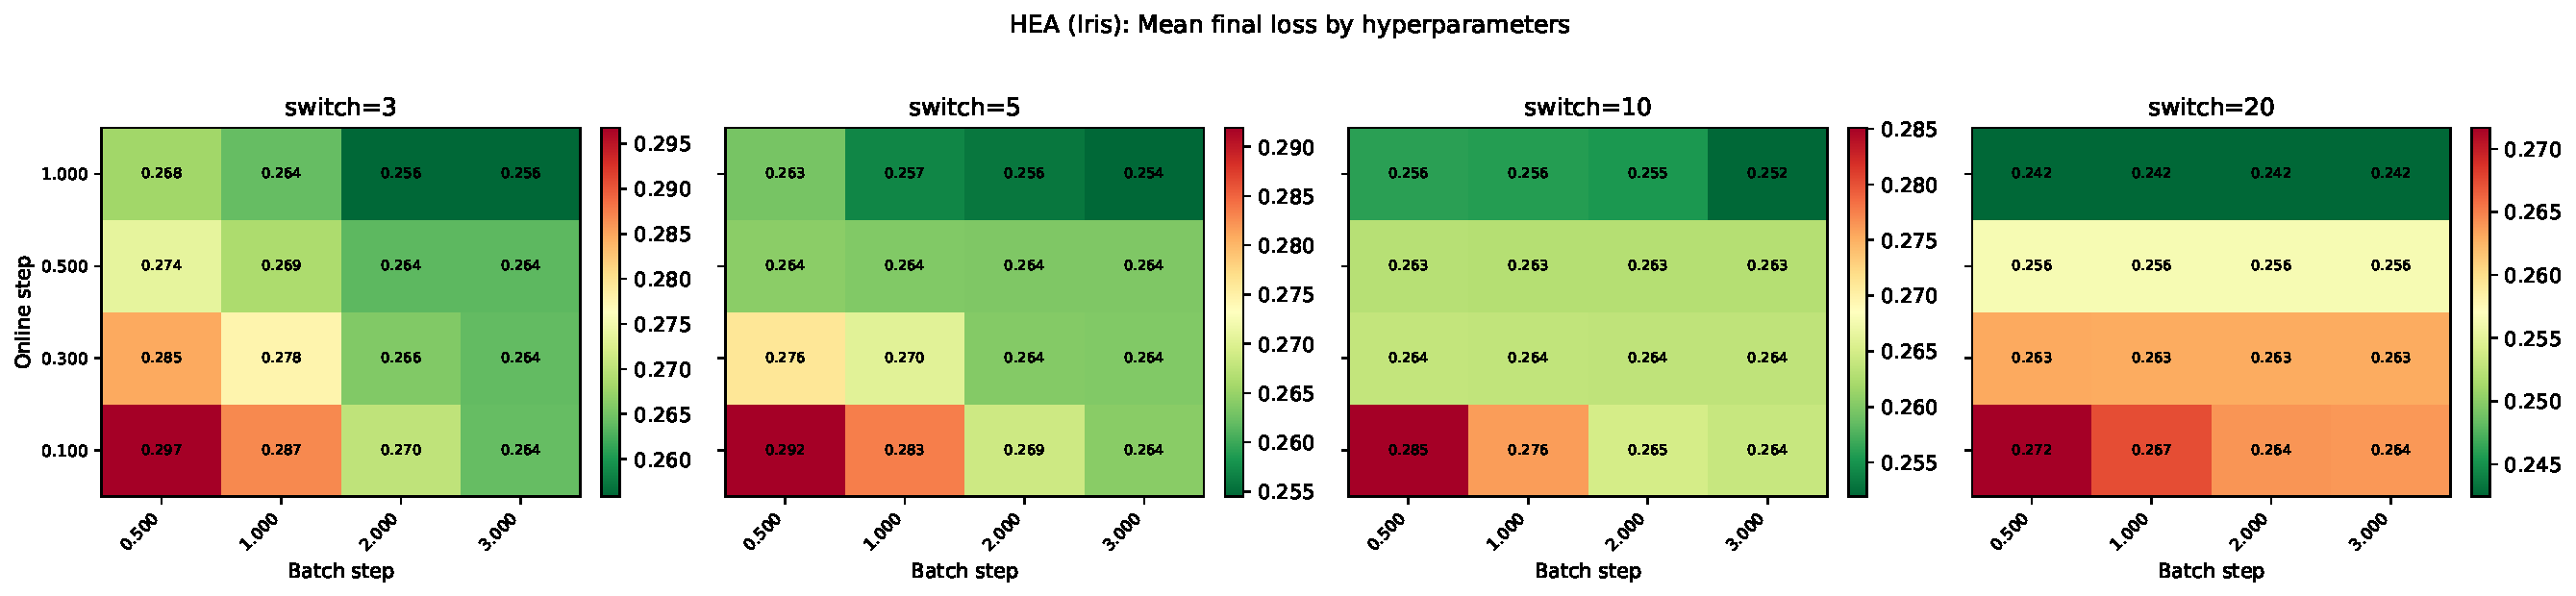
\includegraphics[width=\linewidth]{figures/sweep_hea_heatmap.pdf}
\caption{HEA (Iris)}
\end{subfigure}
\hfill
\begin{subfigure}{0.32\textwidth}
\centering
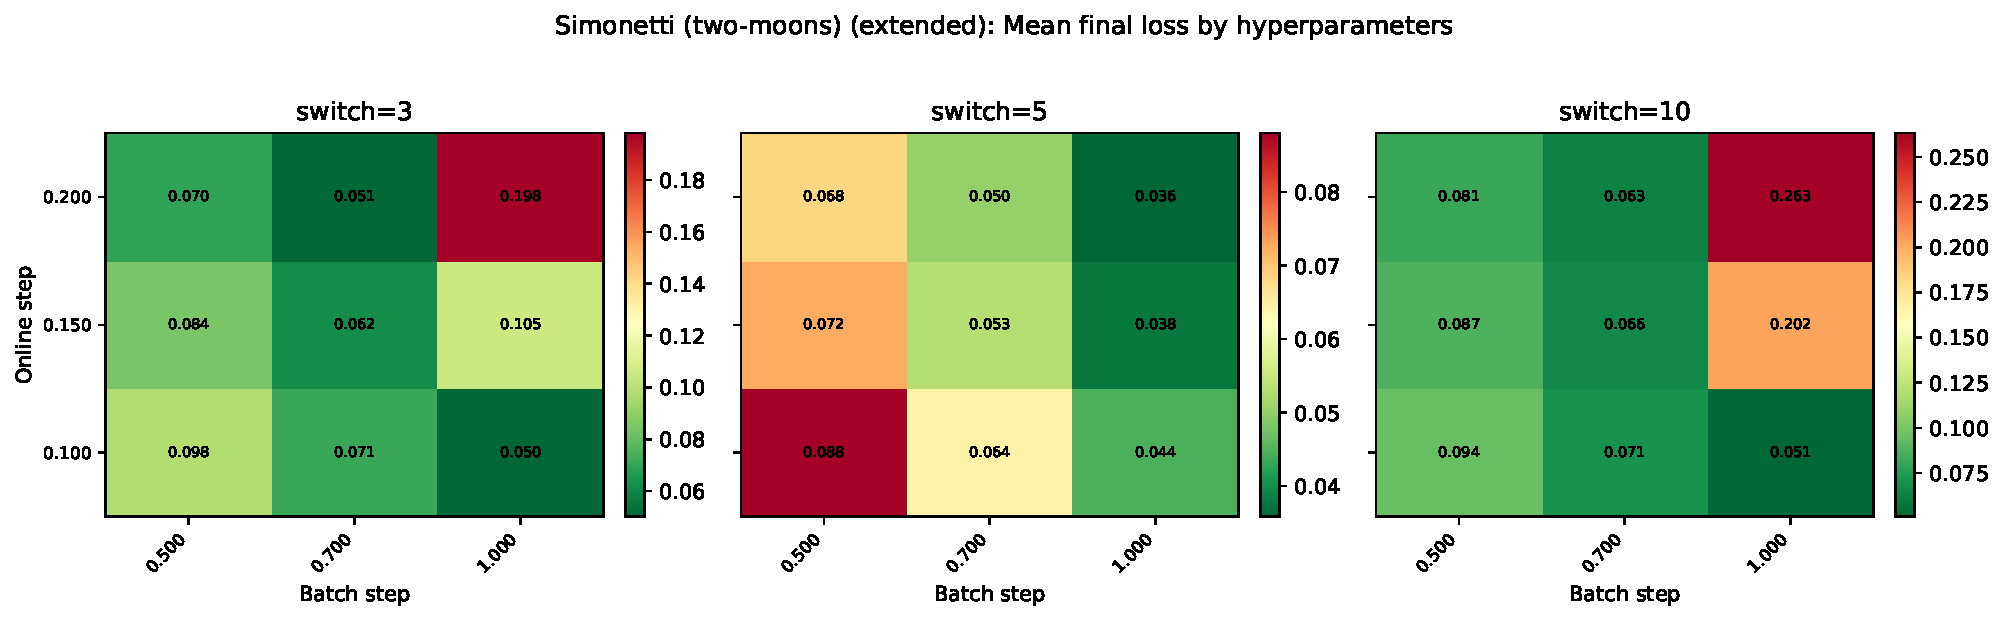
\includegraphics[width=\linewidth]{figures/sweep_simonetti_extended_heatmap.pdf}
\caption{Simonetti}
\end{subfigure}
\hfill
\begin{subfigure}{0.32\textwidth}
\centering
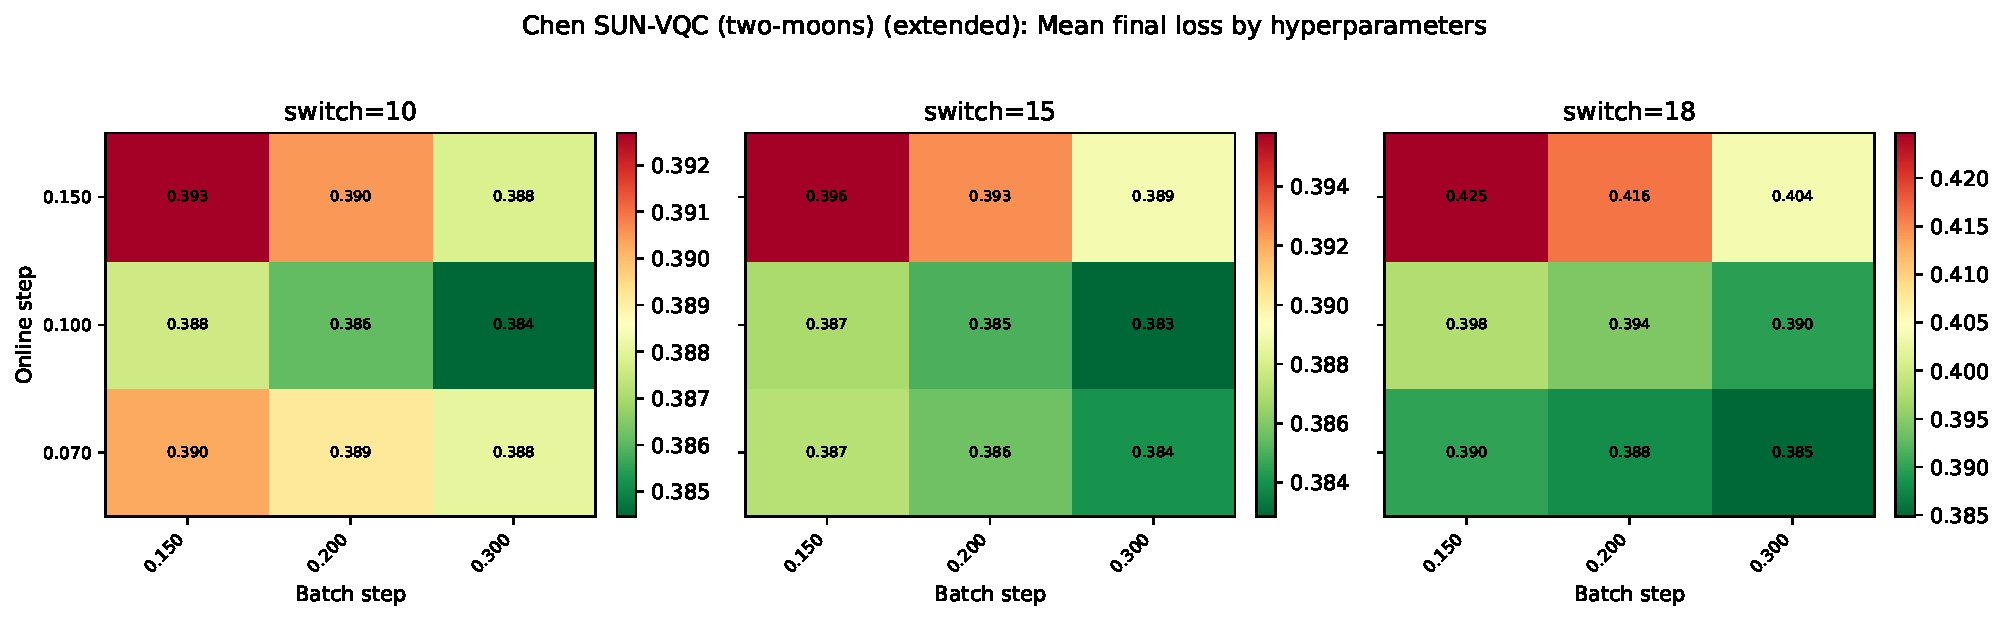
\includegraphics[width=\linewidth]{figures/sweep_chen_extended_heatmap.pdf}
\caption{Chen SUN-VQC}
\end{subfigure}
\caption{Hybrid Krotov tuning landscapes across the three models. The good region is broad on HEA, extremely narrow on Simonetti, and moderately broad on Chen. This visualizes why hybrid Krotov must be presented as a model-dependent optimizer rather than a one-setting universal method.}
\label{fig:hybrid_heatmaps}
\end{figure*}

The sweeps also reveal striking differences in sensitivity.
L-BFGS-B is essentially flat across its tested \texttt{maxcor} and \texttt{gtol} values on all three models.
By contrast, Hybrid Krotov, Adam, and QNG can all improve materially after tuning, with the strongest sensitivity appearing on Simonetti.
In particular, the extended hybrid sweep shows that Simonetti prefers a very short online phase and a much larger batch step than suggested by the original default grid, while Chen prefers a later switch and moderate step sizes.

Finally, motivated by the continuous-time shape factor \(S(t)\), we ran an exploratory discrete-scaling follow-up for hybrid Krotov on the Chen model. The tested factors included adaptive clipping and smoothing based on update magnitude, as well as metadata-based layer scales. The best adaptive setting (clip \(\tau=0.3\), active in both phases, with a \(1.5\times\) step multiplier) reached \(0.3823 \pm 0.008\) over five seeds, and the best metadata-based setting reached \(0.3827 \pm 0.010\). Both are statistically indistinguishable from the best unscaled tuned hybrid result \(0.3828 \pm 0.010\). We therefore treat \(S_k\)-scaling as a mild secondary refinement rather than as a new central mechanism.

\section{Discussion}

The experiments support a more specific story than a generic ``new optimizer beats the baselines'' claim.
The main two-moons HEA benchmark explains the mechanism of the method: online Krotov is most useful as a short, aggressive transient, whereas batch Krotov is most useful as a stable refinement regime.
The hybrid schedule works because it combines these two behaviors.

The tuned cross-model comparison then answers the harder and scientifically more relevant question of competitiveness.
Here the results are clearly architecture-dependent.
On HEA (Iris), Hybrid Krotov and Adam are statistically tied on final loss after tuning, even though the fixed-setting Iris benchmark still favors Hybrid Krotov on threshold speed.
On Chen SUN-VQC, Hybrid Krotov becomes the best tuned optimizer and therefore provides the strongest evidence in the paper that the structured update can beat strong first-, second-, and geometry-aware baselines on a genuinely gate-centric model.
On Simonetti, by contrast, L-BFGS-B is dominant and Hybrid Krotov remains inferior even after tuning, although the gap is far smaller than in the untuned comparison; a short hybrid-Adam warmup further strengthens the Adam-family baseline there.
The follow-up tests also sharpen what does \emph{not} work: hybrid QNG brings no advantage in this study, and a stochastic-to-quasi-Newton L-BFGS-B warm-start would not be a like-for-like baseline because it changes the curvature-memory mechanism rather than merely retuning the optimizer.

This architecture dependence should be understood as a feature of the evidence rather than as a weakness to be concealed.
The present results do not support the claim that Hybrid Krotov is a universal replacement for Adam, L-BFGS-B, or QNG.
They do support the narrower and more credible claim that Hybrid Krotov is a promising structured optimizer niche for gate-centric QML models where circuit propagation structure can be exploited effectively.

Several limitations remain.
First, all experiments are still simulator-based and relatively small in scale.
Second, the theory in this paper covers the batch method and the post-switch phase of the hybrid method, but not the online stale-adjoint phase where the largest empirical oscillations occur.
Third, the sweep-based comparisons use only three seeds per configuration for the literature-inspired models, so the tuned rankings should be interpreted as strong evidence rather than as a final statistical verdict.
Fourth, the present work still does not address shot noise, hardware noise, or sampling-limited gradient estimation; these remain important future tests.

\section{Conclusion}

We have introduced a Krotov-inspired discrete adjoint optimizer for quantum machine learning and studied a hybrid online-to-batch schedule. The method is motivated by a direct structural analogy between continuous-time optimal control and parameterized quantum circuits: forward trajectories become forward gate states, backward costates become backward gate sensitivities, and local control updates become gate-wise parameter updates.

On the theoretical side, we showed that for fixed-generator variational gates and terminal-state losses, the batch Krotov direction is the exact gradient of the empirical loss. This yields monotonic descent and convergence of batch Krotov under standard smoothness assumptions, and convergence of the tail of hybrid Krotov after a finite switch to the batch phase.

On the empirical side, the updated results support a precise and restrained optimizer claim.
The original two-moons HEA benchmark shows why the hybrid schedule is attractive in the first place: it couples the fast basin-entry behavior of online Krotov with the stable late-stage refinement of batch Krotov.
The new Iris benchmark shows that this behavior is not unique to one synthetic dataset.
Most importantly, the tuned cross-optimizer sweeps sharpen the scientific conclusion: Hybrid Krotov is best on the Chen SUN-VQC, statistically tied with the best Adam-family result on HEA (Iris), and decisively outperformed by L-BFGS-B on the Simonetti hybrid classifier. A targeted hybrid-Adam follow-up further improves Simonetti, whereas analogous hybrid-QNG trials bring no benefit.

Taken together, these results position Hybrid Krotov not as a universal optimizer, but as a structured, architecture-dependent method whose advantages are clearest on gate-centric models and whose practical value is best understood through careful tuning rather than one-size-fits-all settings.

\section*{Acknowledgments}
% TODO: Add acknowledgments.

\bibliography{bib.bib}

\appendix

\section{Proof of the exact-gradient representation theorem}

\begin{theorem}[Exact gradient representation of the batch Krotov direction]
\label{thm:exact_gradient_krotov_appendix}
Let
\[
F(\bm{\theta})=\frac{1}{N}\sum_{n=1}^N L_n(\bm{\theta})
\]
be the empirical loss of a parametrized quantum model, where for each sample \(n\),
\[
L_n(\bm{\theta})=\ell\bigl(p_n(\bm{\theta}),y_n\bigr),
\]
and the final quantum state is
\[
|\psi_{n,M}(\bm{\theta})\rangle
=
U_M(\theta_M)\cdots U_1(\theta_1)|\psi_{n,0}\rangle.
\]
For \(k=1,\dots,M\), define the forward states
\[
|\psi_{n,k}(\bm{\theta})\rangle
=
U_k(\theta_k)\cdots U_1(\theta_1)|\psi_{n,0}\rangle,
\qquad
|\psi_{n,0}(\bm{\theta})\rangle:=|\psi_{n,0}\rangle.
\]

Assume that each trainable gate is of the form
\[
U_k(\theta_k)=\exp\!\left(-\frac{i}{2}\alpha_k(\theta_k,x_n)\,G_k\right),
\]
where \(G_k\) is a fixed Hermitian operator, independent of \(\theta_k\), and
\(\alpha_k(\theta_k,x_n)\) is continuously differentiable in \(\theta_k\).

Assume furthermore that, for each sample \(n\), the loss \(L_n(\bm{\theta})\) depends on the
circuit only through the final state \( |\psi_{n,M}(\bm{\theta})\rangle \), and that the terminal costate
\[
|\chi_{n,M}(\bm{\theta})\rangle
\]
is defined by the first-variation identity
\[
\delta L_n(\bm{\theta})
=
2\,\mathrm{Re}\,\langle \chi_{n,M}(\bm{\theta})\mid \delta\psi_{n,M}(\bm{\theta})\rangle
\]
for every variation \(|\delta\psi_{n,M}(\bm{\theta})\rangle\) of the final state.

Finally, define the backward-propagated costates
\[
|\chi_{n,k}^{\mathrm{after}}(\bm{\theta})\rangle
=
U_{k+1}(\theta_{k+1})^\dagger\cdots U_M(\theta_M)^\dagger
|\chi_{n,M}(\bm{\theta})\rangle,
\qquad k=1,\dots,M.
\]

Then, for every sample \(n\) and every gate parameter \(\theta_k\),
\[
\frac{\partial L_n}{\partial \theta_k}(\bm{\theta})
=
2\,\mathrm{Re}\!\left\langle
\chi_{n,k}^{\mathrm{after}}(\bm{\theta})
\middle|
\frac{\partial U_k}{\partial \theta_k}(\theta_k)
\middle|
\psi_{n,k-1}(\bm{\theta})
\right\rangle.
\]
Equivalently,
\[
\frac{\partial L_n}{\partial \theta_k}(\bm{\theta})
=
\frac{\partial \alpha_k}{\partial \theta_k}(\theta_k,x_n)\,
2\,\mathrm{Re}\!\left\langle
\chi_{n,k}^{\mathrm{after}}(\bm{\theta})
\middle|
\left(-\frac{i}{2}G_k\right)
\middle|
\psi_{n,k}(\bm{\theta})
\right\rangle.
\]
Consequently, the batch Krotov direction
\[
d_k(\bm{\theta})
:=
\frac{1}{N}\sum_{n=1}^N
\frac{\partial \alpha_k}{\partial \theta_k}(\theta_k,x_n)\,
2\,\mathrm{Re}\!\left\langle
\chi_{n,k}^{\mathrm{after}}(\bm{\theta})
\middle|
\left(-\frac{i}{2}G_k\right)
\middle|
\psi_{n,k}(\bm{\theta})
\right\rangle
\]
coincides with the exact partial derivative of the empirical loss:
\[
d_k(\bm{\theta})=\frac{\partial F}{\partial \theta_k}(\bm{\theta}).
\]
Hence
\[
d(\bm{\theta})=\nabla F(\bm{\theta}).
\]
\end{theorem}

\begin{proof}
Fix a sample \(n\) and a parameter index \(k\).
By definition of the forward states,
\[
|\psi_{n,M}(\bm{\theta})\rangle
=
U_M(\theta_M)\cdots U_{k+1}(\theta_{k+1})
U_k(\theta_k)
|\psi_{n,k-1}(\bm{\theta})\rangle.
\]
Differentiating with respect to \(\theta_k\) yields
\[
\frac{\partial}{\partial \theta_k}|\psi_{n,M}(\bm{\theta})\rangle
=
U_M(\theta_M)\cdots U_{k+1}(\theta_{k+1})
\frac{\partial U_k}{\partial \theta_k}(\theta_k)
|\psi_{n,k-1}(\bm{\theta})\rangle.
\]

Since \(L_n(\bm{\theta})\) depends on the circuit only through the final state and the terminal
costate is defined by
\[
\delta L_n(\bm{\theta})
=
2\,\mathrm{Re}\,\langle \chi_{n,M}(\bm{\theta})\mid \delta\psi_{n,M}(\bm{\theta})\rangle,
\]
we may apply this identity to the variation induced by changing \(\theta_k\). Thus
\[
\frac{\partial L_n}{\partial \theta_k}(\bm{\theta})
=
2\,\mathrm{Re}\!\left\langle
\chi_{n,M}(\bm{\theta})
\middle|
\frac{\partial \psi_{n,M}}{\partial \theta_k}(\bm{\theta})
\right\rangle.
\]
Substituting the previous expression gives
\[
\frac{\partial L_n}{\partial \theta_k}(\bm{\theta})
=
2\,\mathrm{Re}\!\left\langle
\chi_{n,M}(\bm{\theta})
\middle|
U_M(\theta_M)\cdots U_{k+1}(\theta_{k+1})
\frac{\partial U_k}{\partial \theta_k}(\theta_k)
\middle|
\psi_{n,k-1}(\bm{\theta})
\right\rangle.
\]

Now use the definition of the backward-propagated costate:
\[
|\chi_{n,k}^{\mathrm{after}}(\bm{\theta})\rangle
=
U_{k+1}(\theta_{k+1})^\dagger\cdots U_M(\theta_M)^\dagger
|\chi_{n,M}(\bm{\theta})\rangle.
\]
Taking adjoints yields
\[
\langle \chi_{n,M}(\bm{\theta})|
\,U_M(\theta_M)\cdots U_{k+1}(\theta_{k+1})
=
\langle \chi_{n,k}^{\mathrm{after}}(\bm{\theta})|,
\]
hence
\[
\frac{\partial L_n}{\partial \theta_k}(\bm{\theta})
=
2\,\mathrm{Re}\!\left\langle
\chi_{n,k}^{\mathrm{after}}(\bm{\theta})
\middle|
\frac{\partial U_k}{\partial \theta_k}(\theta_k)
\middle|
\psi_{n,k-1}(\bm{\theta})
\right\rangle.
\]

Now use the gate parametrization
\[
U_k(\theta_k)=\exp\!\left(-\frac{i}{2}\alpha_k(\theta_k,x_n)\,G_k\right).
\]
Because \(G_k\) is independent of \(\theta_k\), the \(\theta_k\)-dependence enters only through
the scalar function \(\alpha_k(\theta_k,x_n)\). Hence the exponent is of the form
\(f(\theta_k)G_k\) with fixed operator \(G_k\), so \(G_k\) commutes with the exponent.
Therefore
\[
\frac{\partial U_k}{\partial \theta_k}(\theta_k)
=
\frac{\partial \alpha_k}{\partial \theta_k}(\theta_k,x_n)
\left(-\frac{i}{2}G_k\right)
U_k(\theta_k).
\]
Substituting this identity yields
\begin{align*}
\frac{\partial L_n}{\partial \theta_k}(\bm{\theta})
&=
\frac{\partial \alpha_k}{\partial \theta_k}(\theta_k,x_n)\,
2\,\mathrm{Re}\!\left\langle
\chi_{n,k}^{\mathrm{after}}(\bm{\theta})
\middle|
\left(-\frac{i}{2}G_k\right)U_k(\theta_k)
\middle|
\psi_{n,k-1}(\bm{\theta})
\right\rangle \\
&=
\frac{\partial \alpha_k}{\partial \theta_k}(\theta_k,x_n)\,
2\,\mathrm{Re}\!\left\langle
\chi_{n,k}^{\mathrm{after}}(\bm{\theta})
\middle|
\left(-\frac{i}{2}G_k\right)
\middle|
\psi_{n,k}(\bm{\theta})
\right\rangle,
\end{align*}
because
\[
|\psi_{n,k}(\bm{\theta})\rangle
=
U_k(\theta_k)|\psi_{n,k-1}(\bm{\theta})\rangle.
\]
This proves the sample-wise identity.

Finally, average over \(n=1,\dots,N\). Since
\[
F(\bm{\theta})=\frac{1}{N}\sum_{n=1}^N L_n(\bm{\theta}),
\]
linearity of differentiation gives
\[
\frac{\partial F}{\partial \theta_k}(\bm{\theta})
=
\frac{1}{N}\sum_{n=1}^N \frac{\partial L_n}{\partial \theta_k}(\bm{\theta}).
\]
Substituting the established formula for each \(\partial L_n/\partial \theta_k\) yields
\[
\frac{\partial F}{\partial \theta_k}(\bm{\theta})=d_k(\bm{\theta}).
\]
Since this holds for every \(k=1,\dots,M\), it follows that
\[
d(\bm{\theta})=\nabla F(\bm{\theta}).
\]
\end{proof}

\begin{remark}
The derivative formula
\[
\frac{\partial U_k}{\partial \theta_k}
=
\frac{\partial \alpha_k}{\partial \theta_k}
\left(-\frac{i}{2}G_k\right)U_k
\]
relies on the fact that \(G_k\) is fixed and independent of \(\theta_k\). If the generator itself
depends on \(\theta_k\), then one must use the general derivative formula for operator exponentials,
and the present proof no longer applies in this form.

Likewise, the first-variation identity
\[
\delta L_n(\bm{\theta})
=
2\,\mathrm{Re}\,\langle \chi_{n,M}(\bm{\theta})\mid \delta\psi_{n,M}(\bm{\theta})\rangle
\]
is valid in the present form because the loss depends only on the final state. If the objective
contains explicit dependence on intermediate states, mid-circuit measurements, or trajectory-level
regularization terms, then the corresponding adjoint construction must be modified.
\end{remark}

\section{Proof of the convergence theorem and hybrid corollary}

\begin{theorem}[Monotonic descent and convergence of batch Krotov]
\label{thm:batch_krotov_convergence_appendix}
Let
\[
F(\bm{\theta})=\frac{1}{N}\sum_{n=1}^N \ell_n(\bm{\theta}), \qquad \bm{\theta}\in\mathbb{R}^p,
\]
be the empirical loss of a parametrized quantum model. Assume that:
\begin{enumerate}
    \item \(F\) is bounded from below;
    \item \(F\) is \(L\)-smooth on the sublevel set
    \[
    \mathcal{L}_0:=\{\bm{\theta}\in\mathbb{R}^p : F(\bm{\theta})\leq F(\bm{\theta}^{(0)})\},
    \]
    i.e.
    \[
    \|\nabla F(\bm{\theta})-\nabla F(\bm{\vartheta})\|
    \leq
    L\|\bm{\theta}-\bm{\vartheta}\|
    \qquad
    \forall \bm{\theta},\bm{\vartheta}\in\mathcal{L}_0;
    \]
    \item the batch Krotov direction coincides with the exact gradient of \(F\).
\end{enumerate}

Consider the batch Krotov iteration
\[
\bm{\theta}^{(m+1)}
=
\bm{\theta}^{(m)}-\eta \nabla F(\bm{\theta}^{(m)}),
\]
with fixed step size \(0<\eta<2/L\).

Then
\begin{enumerate}
    \item[\rm(i)] \(F(\bm{\theta}^{(m)})\) is monotonically nonincreasing and
    \[
    F(\bm{\theta}^{(m+1)})
    \leq
    F(\bm{\theta}^{(m)})
    -
    \eta\left(1-\frac{L\eta}{2}\right)\|\nabla F(\bm{\theta}^{(m)})\|^2;
    \]
    \item[\rm(ii)]
    \[
    \sum_{m=0}^{\infty}\|\nabla F(\bm{\theta}^{(m)})\|^2<\infty;
    \]
    \item[\rm(iii)]
    \[
    \|\nabla F(\bm{\theta}^{(m)})\|\to 0
    \qquad \text{as } m\to\infty;
    \]
    \item[\rm(iv)] every accumulation point of \((\bm{\theta}^{(m)})_{m\geq 0}\) is stationary.
\end{enumerate}
If, in addition, the sequence \((\bm{\theta}^{(m)})_{m\geq 0}\) is bounded and \(F\) satisfies the Kurdyka--\L{}ojasiewicz property on \(\mathcal{L}_0\), then the whole sequence converges to a single stationary point.
\end{theorem}

\begin{proof}
By Assumption (iii), the batch Krotov iteration is exactly gradient descent:
\[
\bm{\theta}^{(m+1)}=\bm{\theta}^{(m)}-\eta \nabla F(\bm{\theta}^{(m)}).
\]
Since \(F\) is \(L\)-smooth on \(\mathcal{L}_0\), the descent lemma gives
\[
F(\bm{\theta}^{(m+1)})
\leq
F(\bm{\theta}^{(m)})
+
\langle \nabla F(\bm{\theta}^{(m)}),\bm{\theta}^{(m+1)}-\bm{\theta}^{(m)}\rangle
+
\frac{L}{2}\|\bm{\theta}^{(m+1)}-\bm{\theta}^{(m)}\|^2.
\]
Substituting
\[
\bm{\theta}^{(m+1)}-\bm{\theta}^{(m)}=-\eta \nabla F(\bm{\theta}^{(m)}),
\]
we obtain
\begin{align*}
F(\bm{\theta}^{(m+1)})
&\leq
F(\bm{\theta}^{(m)})
-
\eta\|\nabla F(\bm{\theta}^{(m)})\|^2
+
\frac{L\eta^2}{2}\|\nabla F(\bm{\theta}^{(m)})\|^2 \\
&=
F(\bm{\theta}^{(m)})
-
\eta\left(1-\frac{L\eta}{2}\right)\|\nabla F(\bm{\theta}^{(m)})\|^2.
\end{align*}
Because \(0<\eta<2/L\), the coefficient
\[
c:=\eta\left(1-\frac{L\eta}{2}\right)
\]
is strictly positive. This proves (i).

Summing from \(m=0\) to \(M\) yields
\[
F(\bm{\theta}^{(M+1)})
\leq
F(\bm{\theta}^{(0)})-c\sum_{m=0}^M \|\nabla F(\bm{\theta}^{(m)})\|^2.
\]
Since \(F\) is bounded below, say by \(F_{\inf}\), we obtain
\[
c\sum_{m=0}^M \|\nabla F(\bm{\theta}^{(m)})\|^2
\leq
F(\bm{\theta}^{(0)})-F_{\inf}.
\]
Letting \(M\to\infty\) gives
\[
\sum_{m=0}^{\infty}\|\nabla F(\bm{\theta}^{(m)})\|^2<\infty,
\]
which proves (ii). In particular,
\[
\|\nabla F(\bm{\theta}^{(m)})\|\to 0,
\]
which proves (iii).

Now let \(\bm{\theta}^{\star}\) be an accumulation point. Then there exists a subsequence
\[
\bm{\theta}^{(m_j)}\to \bm{\theta}^{\star}.
\]
Since \(\nabla F\) is continuous,
\[
\nabla F(\bm{\theta}^{\star})
=
\lim_{j\to\infty}\nabla F(\bm{\theta}^{(m_j)})
=
0,
\]
using (iii). Hence \(\bm{\theta}^{\star}\) is stationary, proving (iv).

If the iterates are bounded and \(F\) satisfies the Kurdyka--\L{}ojasiewicz property, the standard KL convergence theorem for descent methods applies, yielding convergence of the entire sequence to a single stationary point.
\end{proof}

\begin{corollary}[Convergence of hybrid Krotov after a finite switch]
\label{cor:hybrid_krotov_convergence_appendix}
Let \((\bm{\theta}^{(m)})_{m\geq 0}\) be generated by a hybrid Krotov method such that there exists a finite switching time \(T<\infty\) with the following property:
\begin{itemize}
    \item for \(m<T\), the iterates are generated by an arbitrary online Krotov phase;
    \item for \(m\geq T\), the iterates are generated by the batch Krotov update
    \[
    \bm{\theta}^{(m+1)}
    =
    \bm{\theta}^{(m)}-\eta \nabla F(\bm{\theta}^{(m)}),
    \]
    with a step size \(0<\eta<2/L\).
\end{itemize}
Assume that the assumptions of Theorem~\ref{thm:batch_krotov_convergence_appendix} hold on the sublevel set
\[
\mathcal{L}_T:=\{\bm{\theta}\in\mathbb{R}^p : F(\bm{\theta})\leq F(\bm{\theta}^{(T)})\}.
\]
Then the tail sequence \((\bm{\theta}^{(m)})_{m\geq T}\) converges to a stationary point under the same boundedness and Kurdyka--\L{}ojasiewicz assumptions.
\end{corollary}

\begin{proof}
Define the shifted sequence
\[
\widetilde{\bm{\theta}}^{(j)}:=\bm{\theta}^{(T+j)}, \qquad j\geq 0.
\]
By construction,
\[
\widetilde{\bm{\theta}}^{(j+1)}
=
\widetilde{\bm{\theta}}^{(j)}-\eta \nabla F(\widetilde{\bm{\theta}}^{(j)}),
\]
with \(0<\eta<2/L\). Thus \((\widetilde{\bm{\theta}}^{(j)})_{j\geq 0}\) is exactly a batch Krotov sequence started from \(\widetilde{\bm{\theta}}^{(0)}=\bm{\theta}^{(T)}\). Applying Theorem~\ref{thm:batch_krotov_convergence_appendix} to the shifted sequence proves the claim.
\end{proof}

\end{document}